\documentclass[12pt]{article}
	\usepackage[danish]{babel}
	\usepackage{tabularx}
	\usepackage{varwidth}
	\usepackage{array}
    \usepackage[margin=1in]{geometry}
    \usepackage{amsmath}
    \usepackage[utf8]{inputenc}
    \usepackage{graphicx}
    \usepackage{fancyhdr}
    \usepackage{lastpage}
    \usepackage[T1]{fontenc}
    \usepackage{amssymb}
    \usepackage{listings}
    \usepackage{minted}
    \usepackage[colorinlistoftodos]{todonotes}
    \usepackage{wrapfig}
    \usepackage{subcaption}
    \usepackage{hyperref}
    \usepackage{todonotes}
    \usepackage[final]{pdfpages}
    \usepackage{parskip}
    \usepackage{float}
    
    \pagestyle{fancy}

    \title{UIS Projektgrundlag }
    \author{Casper Bresdahl whs715\\ Torben Olai Milhøj vrw704\\ Sarah Willumsen zql291\\ Mads Rosenlund Jensen lfh632\\}
    \date{}
    \begin{document}
        \maketitle
        \thispagestyle{empty}
        \cfoot{Page \thepage ~of \pageref{LastPage}}
        %Af en eller anden grund stod der INDHOLD i sidehovedet, disse tre linjer fjerner dette
        \chead{}
        \lhead{}
        \rhead{}
        %Fjerner linjen i sidehovedet
        \renewcommand{\headrulewidth}{0pt}

        \tableofcontents
        \newpage
        \setcounter{page}{1}
        \section{Projektets præmisser}
\subsection{Baggrund}
Sundhedsplatformen blev valgt af regionerne i november 2013 og er bliver udviklet af det amerikanske selskab Epic. Sundhedsplatformen er bindeled mellem mange undersystemer og samler alle de funktioner som de 44000 danske sundhedsprofessionelle benytter mest. I Danmark bliver Sundhedsplatformen benyttet på 17 sygehuse eller hospitaler til 2.5 millioner borgere i Region Sjælland og Region Hovedstaden. På verdensplan er Sundhedsplatformen i drift på 1100 hospitaler og omfatter 172 millioner patienter.\\
Patienter har adgang til Sundhedsplatformen gennem 'Min Sundhedsplatform' (Min SP) som vores projekt vil fokusere på. Gennem Min SP kan patienter skrive beskeder til ambulatorier, anmode om at aflyse og få nye tider, se prøvesvar og få adgang til dele af ens journaler. Min SP og Sundhedsplatformen er stadig under udvikling og læger, sygeplejersker, it-specialister og projektledere i Region Sjælland og Hovedstaden tilpasser og opdatere løbende systemerne til fremtidens behov for behandlinger.
\todo{Tilføj afsnit om samarbejdspartnere / hospitaler}
\subsection{Opgave og formål}
Projektets overordnede formål vil være, at i samarbejde med sundhedspersonale, diabetikere og region hovedstaden at realisere visionen om forbedringer til 'Min Sundhedsplatform'. Ved projektets begyndelse fandt vi følgende cases som vi mente ville være forbedringer til 'Min Sundhedsplatform'.
\subsubsection{Receptfornyelse}
Vi mente at netop det at skulle fornye sin recept var en enkel process som i forvejen kan gøres online men på sundhed.dk. Ved at gøre det muligt at fornye sin recept på Min Sundhedsplatform ville man samle flere (hvis ikke alle) arbejdsprocessor til den samme side for diabetikere, og det vil derfor ikke kræve at diabetikere skal sætte sig ind i flere sider for at få behandling.
\subsubsection{Læring og videnscenter}
Vi identificerede at der ikke var meget almen information omkring diabetes og patienters sygdom generelt på Min Sundhedsplatform. Vi ville derfor gerne kigge videre på mulighederne i at samle viden omkring sygdommen, såsom hvad man skal gøre hvis man oplever situation x eller y. Ved at samle information og viden på Min Sundhedsplatform vil man give diabetikeren et enkelt sted hvor de burde kunne finde al den nødvendige information. Dette videnscenter vil hovedsagligt henvende sig til den nye eller uerfarne diabetiker som måske lige er blevet oplært i sin sygdom. Denne udvidelse af Min Sundhedsplatform ville også kunne tjene til motivation frem mod diabetikerens nye livsstil.
\subsubsection{Socialt samlingssted}
Ved at inkorporere et socialt samlingssted på Min Sundhedsplatform ville man kunne forbinde mennesker med andre som deler de samme bekymringer ved at have fået konstateret diabetes. Den sociale del kunne bestå af både større grupper hvor man kan dele viden og erfaringer eller det kunne bestå af mindre men mere intime grupper som måske ønsker at mødes og være sammen. Forumet ville lægge op til at dele viden og erfaring, og motivere hinanden. Man kunne forstille sig at en lille gruppe ældre kunne finde sammen nogle gange om ugen og cykle en tur og på den måde motivere hinanden til den ændrede livsstil.
\subsubsection{Forberedelse af fremtiden}
I fremtiden vil vi helt sikkert se teknologisk fremgang i forhold til behandlingen af diabetes. Vi forestiller os at et fremtidigt initiativ kunne være at implementere en chip hos patienterne som hele tiden måler blodsukkeret. Denne case ville fokusere på hvordan man i fremtiden ville kunne benytte sig af det potentiale som det ville være hvis diabetikerens blodsukker hele tiden blev målt, og hvordan det potentiale kunne bruges af Min Sundhedsplatform. Man kunne forestille sig at ved hjælp af machine learning og databehandling kunne man forudse unormale ændringer i blodsukkeret og advare diabetikeren, for eksempel gennem en app, og relevant sundhedspersonale.\\\\
Blandt de fire cases valgte vi at skrive et spørgeskema som gav os mulighed for at se om der er nogen relevans for vores forslag. Gennem princippet om brugerindragelse kom vi frem til at arbejde videre med \todo{Videre arbejde} 
\subsection{Tekniske rammer}
De tekniske rammer udgøres af muligheden for at forbinde den forbedrede Min Sundhedsplatform sammen med Sundhedsplatformen, og at gøre forbedringen overskuelig og forståelig for alle brugere. Vi forudser ingen problemer med at koble Min Sundhedsplatform sammen med Sundhedsplatformen efter projektets realisering. Den eneste tekniske ramme vil derfor bestå af at få realiseret projektet på en hensynsfuld måde således at det kan forstås af både unge og ældre.
\subsection{Kritiske faktorer}
For at projektet skal kunne realiseres og blive en succes, kræves det at de kritiske faktorer kan løses. Vi har identificeret at projektet ikke vil blive en succes hvis realiseringen ikke er i øje med patienterne. Da diabetikere findes i mange aldre, vil det derfor kræve at brugervenligheden og tilgængeligheden tænkes ind i projektet i en meget væsentlig stil.
        \section{Strategisk analyse}
\begin{figure}[H]
	\centering
	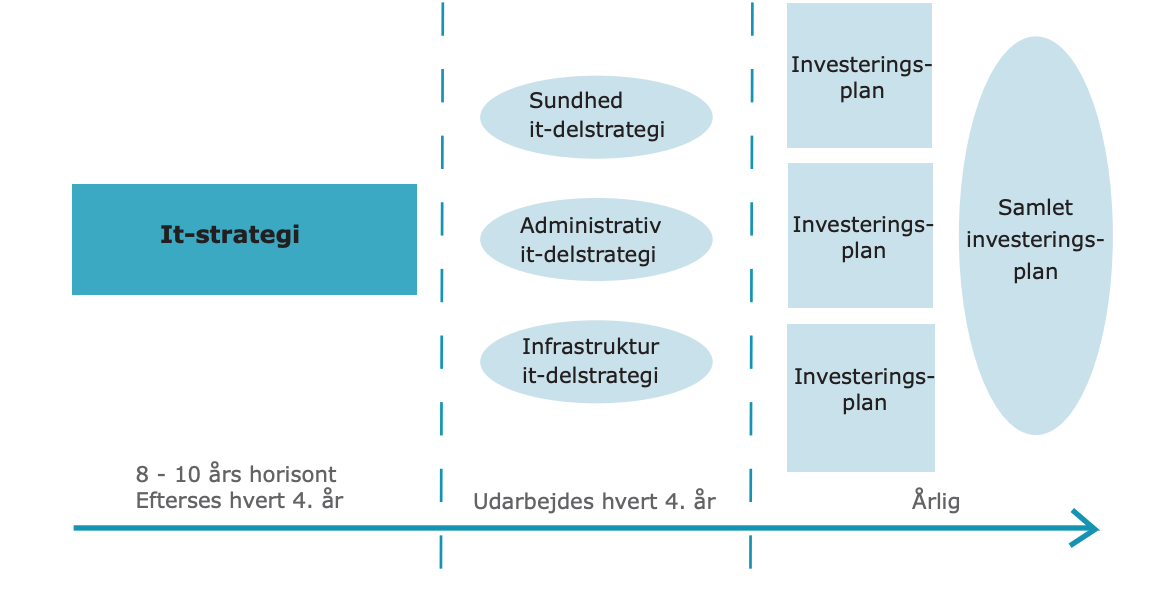
\includegraphics[width=\linewidth]{Materials/Strategy}
	\caption{It-strategien for Region Sjælland og de tilhørende it-delstrategier}
\end{figure}
Ovenfor ses Region Sjællands it strategi, og hvordan den er bygget op. Den overordnede it strategi udgør sammen med delstrategierne rammerne for investeringsplanerne som efterfølgende financierer strategierne. Som det ses er tidshorisonten for den overordnede it strategi på otte til ti år. Denne tilgang er taget for at sikre ambitionsniveauet for strategien kan realiseres over flere delstrategiperioder således at regionen løbende kan få et indtryk af den aktuelle situation.
\subsection{IT Strategien}
Nogle af de vigtigste målsætninger for den overordnede it strategi er:
\begin{enumerate}
	\item Regionen ønsker at skabe en sammenhængende og effektiv virksomhed gennem øget samarbejde både internt men også med samarbejdspartnere og borgere.
	\item Regionen vil have fuldt udbytte af sine investeringer, og de nye løsninger skal bruges i deres fulde omfang.
	\item Regionen vil begrænse risici involveret i at indføre nye it løsninger og vil derfor tage ved lære af andres viden og erfaringer. Det er derfor at foretrække hvis de nye systemer er efterprøvede af andre organisationer i eller uden for landet.
	\item De administrative og kliniske arbejdspladser skal have samlet adgang og samlet præsentation til al relevant data uanset kilde og teknologi. De skal have adgang fra en flerhed af mobile enheder. Der skal desuden være større anvendelse af data i eksisterende og kommende systemer.
	\item Regionen har en målsætning om at de administrative og kliniske arbejdspladser skal være papirløse. Dette skal realiseres ved at automatisere, forenkle og standardisere opgavevaretagelse.
	\item De løsninger som tages i brug skal være brugervenlige og intuitive.
	\item Regionen har en målsætning om at borgere, patienter,
	pårørende og samarbejdspartnere i så høj grad som muligt kan betjene dem selv uden at gå på kompromis med kvalitet og service. Målet er, at disse grupper skal opleve en bedre servicegrad, samtidig med at regionen reducerer sit ressourceforbrug.
	\item Regionen ønsker én arbejdsopgave til ét system. Men det er samtidigt vigtigt med systemer som kan hente information fra andre systemer.
\end{enumerate}
\subsection{Sundheds-it}
Nogle af de vigtigste målsætninger for sundheds it strategien er:
\begin{enumerate}
	\item Regionen har en målsætning om at give ensartede oplevelser og behandling uanset geografi.
	\item Regionen ønsker at den enkelte kliniker skal kunne få et samlet, mobilt og nemt tilgængeligt overblik over de opgaver og de patienter som den enkelte kliniker tildeles eller har kontakt til. I princippet skal en kliniker kunne
	trække 'glaspladen' op af lommen og få fuldt overblik over egne opgaver og alle relevante kliniske data og billeder fra alle systemer.
	\item Gennem implementering af it systemer ønsker regionen at understøtte driften og sikre effektivisering af ressourceanvendelsen.
	\item Telemedicin skal optimere patientforløb i forhold til accelerering, adgang til relevant ekspertise, diagnostik, behandling og kontinuitet. 
\end{enumerate}
\subsection{Administrativ-it}
Nogle af de vigtigste målsætninger for den administrative it strategi er:
\begin{enumerate}
	\item Regionen vil skabe en sammenhængende, effektiv og papirløs administration gennem automatisering, procesunderstøttelse og digitalisering af arbejdsgange.
	\item Regionen ønsker realtidsledelsesinformation som skal tage afsæt i driften.
	\item Regionens kommunikative mål er ensartethed uanset geografi og at de kommunikative it løsninger skal være mobile.
\end{enumerate}
\subsection{It-infrastruktur}
Nogle af de vigtigste målsætninger for it-infrastruktur strategien er:
\begin{enumerate}
	\item Regionens infrastruktur skal være sikker, enkel, let og stabilt tilgængelig og med ubegrænset kapacitet set fra brugerens synspunkt.
	\item Regionen vil løbende tage nye systemer i brug, og ønsker derfor løsninger som der kan udvides.
	\item Brugeren skal kunne finde løsninger i samme brugervendte arbejdsgange, uden at brugerne skal opleve behov for at navigere mellem forskellige løsninger. Regionen ønsker systemer som kan hente information fra andre systemer således at brugeren kun skal henvende sig et enkelt sted.
	\item Regionen ønsker integrerede selvbetjenings løsninger.
\end{enumerate}


Al information i kapitlet er taget fra Region Sjællands egen publikation af deres it strategi\footnote{\url{https://www.regionsjaelland.dk/publikationer/Documents/it-strategi-region-sjaelland.dk.pdf}}.

\subsection{Problemer og behov}
Ud fra de ovenstående mål, ser vi at regionen finder det problematisk at klinikere ikke har det store overblik ved hånden hele tiden. De ønsker løsninger som er mobile og kan skabe overblik på kryds af alle systemer. De møder problemer med ressourceallokering, og hvordan de effektivt benytter de ressourcer de har til rådighed.\\
De har behov for systemer som er sikre og intuitive for brugerne, og som brugeren selv kan betjene. De har behov for et samlet system hvor brugeren kan finde al nødvendig information. De har behov for systemer som er afprøvede og testede i drift. Der er behov for at de it løsninger som bliver taget i brug kan udvides.
        \section{Organisering}
\subsection{Projekt organisering}
Projektet består af projektgruppen og styregruppen.\\
Projektgruppen består af Casper Bresdahl, Sarah Willumsen, Torben Milhøj og Mads Rosenlund og har til opgave at aktivt arbejde på design løsninger til projektet samt at levere resultater for tidligere aftalte baselines.\\
Styregruppen består af TA teamet og Finn Kensing og har til opgave at svare på tvivlsspørgsmål fra projektgruppen, tillade projektgruppens forslag og dobbelttjekke den information som projektgruppen giver.
\subsection{Interessenter}
Vi har identificeret følgende interessenter:
\begin{enumerate}
	\item \textbf{Diabetikerne.}\\
	Diabetikerne er de direkte brugere af projektet og dem som projektet skal hjælpe og skræddersys til.
	\item \textbf{Region Hovedstaden og Sjælland.}\\
	Skulle projektet realiseres vil det være Region Hovedstaden og Region Sjælland som ville skulle finansiere og starte udviklingen af projektet.
	\item \textbf{Sundhedsministeren.}\\
	Skulle projektet vise sig at blive en stor succes kunne man forestille sig at det ville blive lanceret i hele landet, og ville derfor skulle involvere sundhedsministeren.
\end{enumerate}
        \section{Metode}
\subsection{Overordnet tilgang}
Tilgangen til projektet er baseret på MUST principperne beskrevet i 'Participatory IT Designing for Business and Workplace Realities'. Ligeledes er de benyttede og de fremtidige redskaber og aktiviteter beskrevet i projektgrundlaget baseret på anbefalinger fra samme bog.\\
Nedenfor findes vores udarbejdede baseline som viser deadlines og produkter for vores projekt. Initiation phase og in-line analysis fasen er blevet lagt sammen, og de aktiviteter beskrevet i denne kombi-fase er blevet udført. Aktiviteterne i de fremtidige faser er foreløbige og stadig til debat hvorvidt de skal ændres. \todo{Ændr engelske begreber?}
\begin{figure}[h!]
	\missingfigure{Billede af Baseline}
	\caption{Udarbejdet baseline}
\end{figure}
Region Sjælland har et strategisk ønske om it systemet skal være gennemtestet samt at opnå fuld tilgængelighed blandt læger og patienter. Af denne årsag ønsker vi at lave en markedsundersøgelse for at komme på sporet. Hertil vil vi benytte os af SWOT-analysen til at visualisere hvorledes analysens elementer vægtes.
Som led i regionens strategi om at klinikere skal have overblik over relevante data og billeder, vil vi arrangere insitu-interview, hvor vi kortlægger hvilke data der er relevante. Insitu-interview vil ligeledes også være relevante ift. patienter og behandlere, for at vi kan nedbringe konsultation- og behandlingstid.   
\newpage
\subsection{Plan}
I den følgende tabel highligther vi nogle af de udførte og fremtidige aktiviteter, og vores målsætninger for dem. De fremtidige aktiviteter er stadig under debat og kan blive ændret undervejs i projektet.
\newcolumntype{M}{>{\begin{varwidth}{6cm}}l<{\end{varwidth}}}
\begin{table}[h!]
	\centering
	\begin{tabularx}{\textwidth}{|X|M|X|}
		\hline
		Aktivitet&Involverede&Resultat af aktivitet\\
		\hline
		Research af diabetes & Projektgruppen & Overordnet viden om diabetes\\
		\hline
		Udspecificering af opgaven & Projektgruppen & Valg af fokus punkter for projektet\\
		\hline
		Baseline plan & Projektgruppen & Udvikling af baseline for projektet\\
		\hline
		Forståelse af Region Hovedstadens og Region Sjællands forretningsstrategi, analyse af kritiske faktorer for projektet og interessantanalyse & Projektgruppen & Overordnet viden om regionernes strategier\\
		\hline
		Valg af deltagere til interviews og kontakt til hospitaler for muligt besøg & Projektgruppen & \\
		\hline
		Arbejde med interview og spørgeskemaer & Projektgruppen & Interview og spørgeskema til deltagere i projektet\\
		\hline
		Udførelse af interviews & Projektgruppen og deltagere & \\
		\hline
		Besøg hos sundhedspersonale med henblik på arbejdsprocessor og in-situ interview(s) & Projektgruppen og deltagere & Forståelse for sundhedspersonalets arbejdsprocessor\\
		\hline
		Undersøgelse af andre lignende designløsninger & Projektgruppen & \\
		\hline
		Præsentation af projekt for styregruppe og Regionerne & Projekt gruppen, Styregruppen og Regionerne & \\
		\hline
		Udvikling af tidlig prototype til præsentation for diabetikere og sundhedspersonale & Projektgruppen og deltagere & Sikre os at vores produkt stadig er i linje med behovet for produktet\\
		\hline
		Sidste detaljer vedrørende projekt og prototype & Projektgruppen & Færdigt projekt\\
		\hline
	\end{tabularx}
	\caption{Overordnet plan for projektet}
\end{table}
\subsection{Teknikker}
Nedenfor vil vi liste de teknikker som vi har og planlægger at benytte i løber af vores projekt.\\ \todo{Ændr engelske begreber?}

\textbf{Initiation and in-line analysis phase:}
\begin{enumerate}
	\item Kapitel 9.1, Baseline planlægning
	\item Kapitel 9.4, Interview / spørgeskema
	\item Kapitel 9.5, Dokument analyse
\end{enumerate}
\textbf{In-depth analysis phase:}
\begin{enumerate}
	\item Kapitel 9.6, Functional analysis
	\item Kapitel 9.7, SWOT analyse
	\item Kapitel 9.8, In-situ interview og observation
\end{enumerate}
\textbf{Innovation phase:}
\begin{enumerate}
	\item Kapitel 7.5, idé udvikling
	\item Kapitel 7.5.5, Identificering af kvalifikationskrav
	\item Kapitel 7.5.6, Konsekvens analyse
	\item Kapitel 9.1.5, Mock-ups og prototyper
\end{enumerate}
        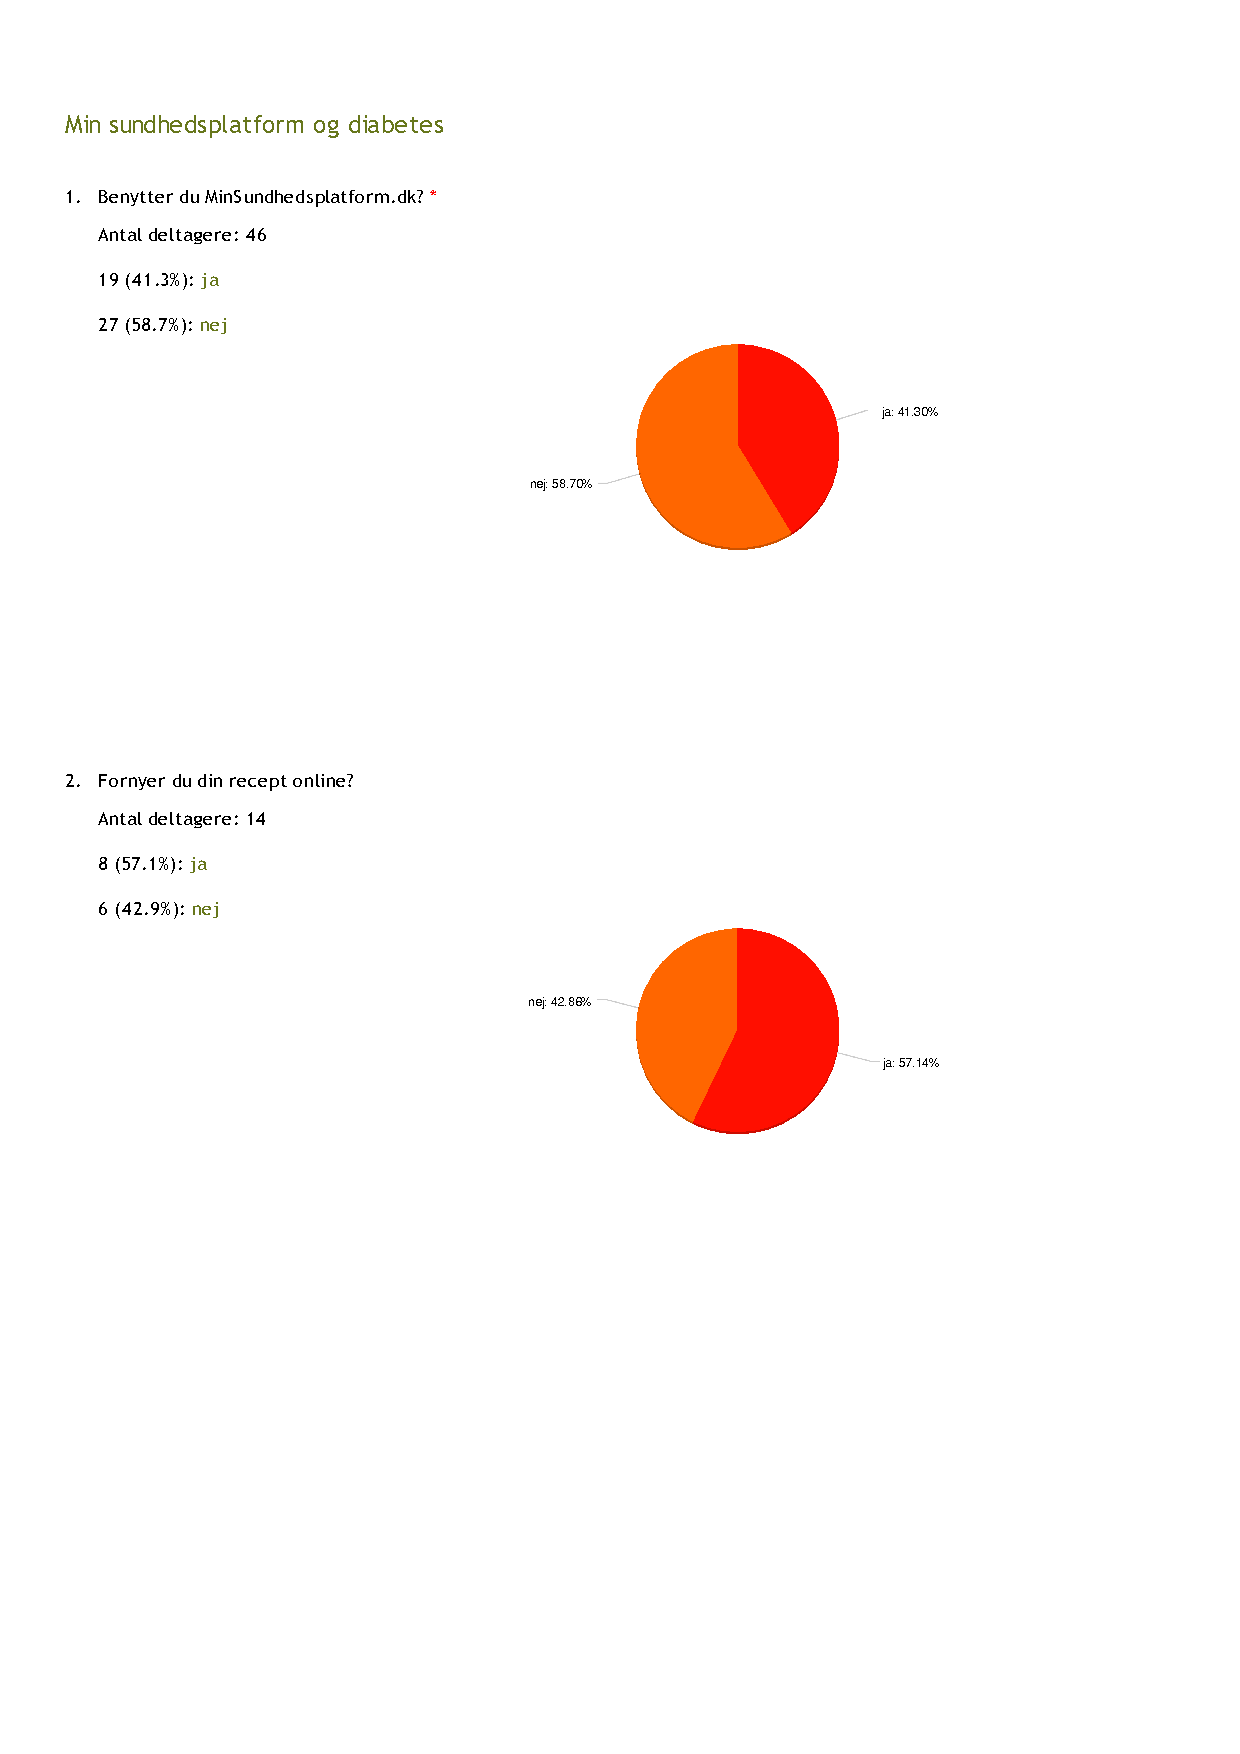
\includepdf[pages=1,pagecommand={\section{Bilag 1} \thispagestyle{empty}}, fitpaper=true, offset=0 -80]{Materials/Questionaire.pdf}
        \includepdf[pages=2-,pagecommand={\thispagestyle{empty}}, fitpaper=true]{Materials/Questionaire.pdf}
        
        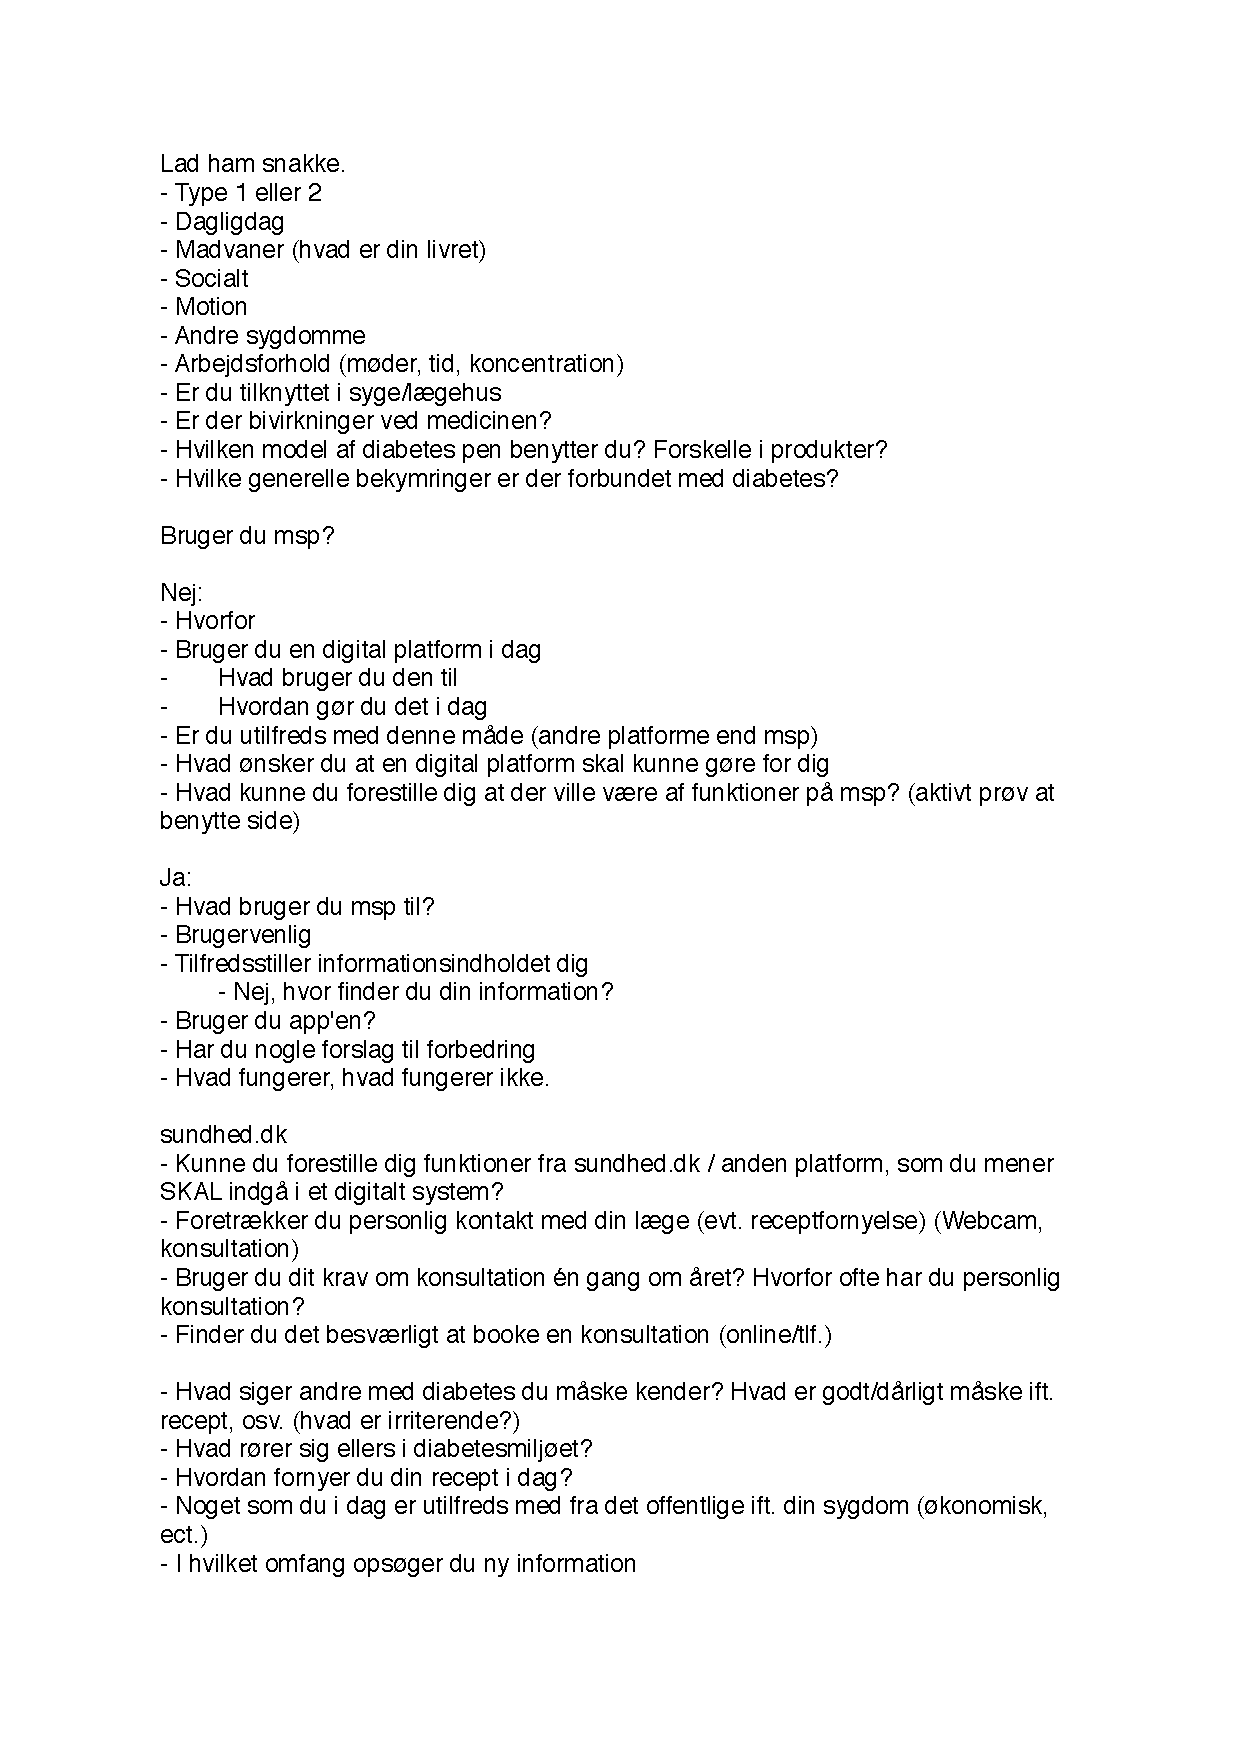
\includepdf[pages=1,pagecommand={\section{Bilag 2} \thispagestyle{empty}}, fitpaper=true, offset=0 -50]{Materials/Interview.pdf}
        \includepdf[pages=2-,pagecommand={\thispagestyle{empty}}, fitpaper=true]{Materials/Interview.pdf}
        \end{document}
